\documentclass[12pt]{article} %Tipo de documento (puede ser book, report, etc.)

\usepackage[utf8]{inputenc} %Codificación de caracteres (UTF-8)
\usepackage{amsmath, amssymb} %Paquetes para expresiones matemáticas
\usepackage{graphicx} %Para insertar imágenes
\usepackage[spanish]{babel} %Optimiza el typesetting para documentos en español
\usepackage[letterpaper, left=1in, right=1in, top=1in, bottom=1in]{geometry}
%Para abarcar más hoja horizontalmente
\usepackage{booktabs} %Optimiza trabajar con tablas y agrega algunos comandos
\usepackage{multirow} %Para crear celdas tabulares que abarcan múltiples filas
\usepackage{float} %Mayor control sobre dónde se colocan las figuras y tablas
\usepackage{caption} %Mayor control de las captions de figuras y tablas
\usepackage{colortbl} %Para colores en tablas
\usepackage{xcolor} %Opcional, pero útil para definir colores personalizados
\definecolor{paleYellow}{RGB}{255, 255, 180} %Ejemplo con amarillo pálido
\usepackage{hyperref}

%Preámbulo
\title{}
\author{Suárez Saldaña, Jorge Alberto \\ Matrícula: 355992}
\date{\today}

\begin{document}
\maketitle

\section{Introducción}
Aquí va la introducción.

\subsection{Figuras}
Algún apartado dentro de la introducción

En la figura \ref{fig:EjemploFigVerb} verás un ejemplo de figura con entorno verbatim 
y en la figura \ref{fig:EjemploFigGraph} verás un ejemplo de figura con includegraphics.

\begin{figure}[H]
  \centering
  \caption{Esta es una figura con verbatim}
  \label{fig:EjemploFigVerb}
  \begin{verbatim}
    Lo que escribas aquí,
      Se escribirá tal cual.
  \end{verbatim}
\end{figure}

\begin{figure}[H]
  \centering
  \caption{Esta es una figura con includegraphics}
  \label{fig:EjemploFigGraph}
  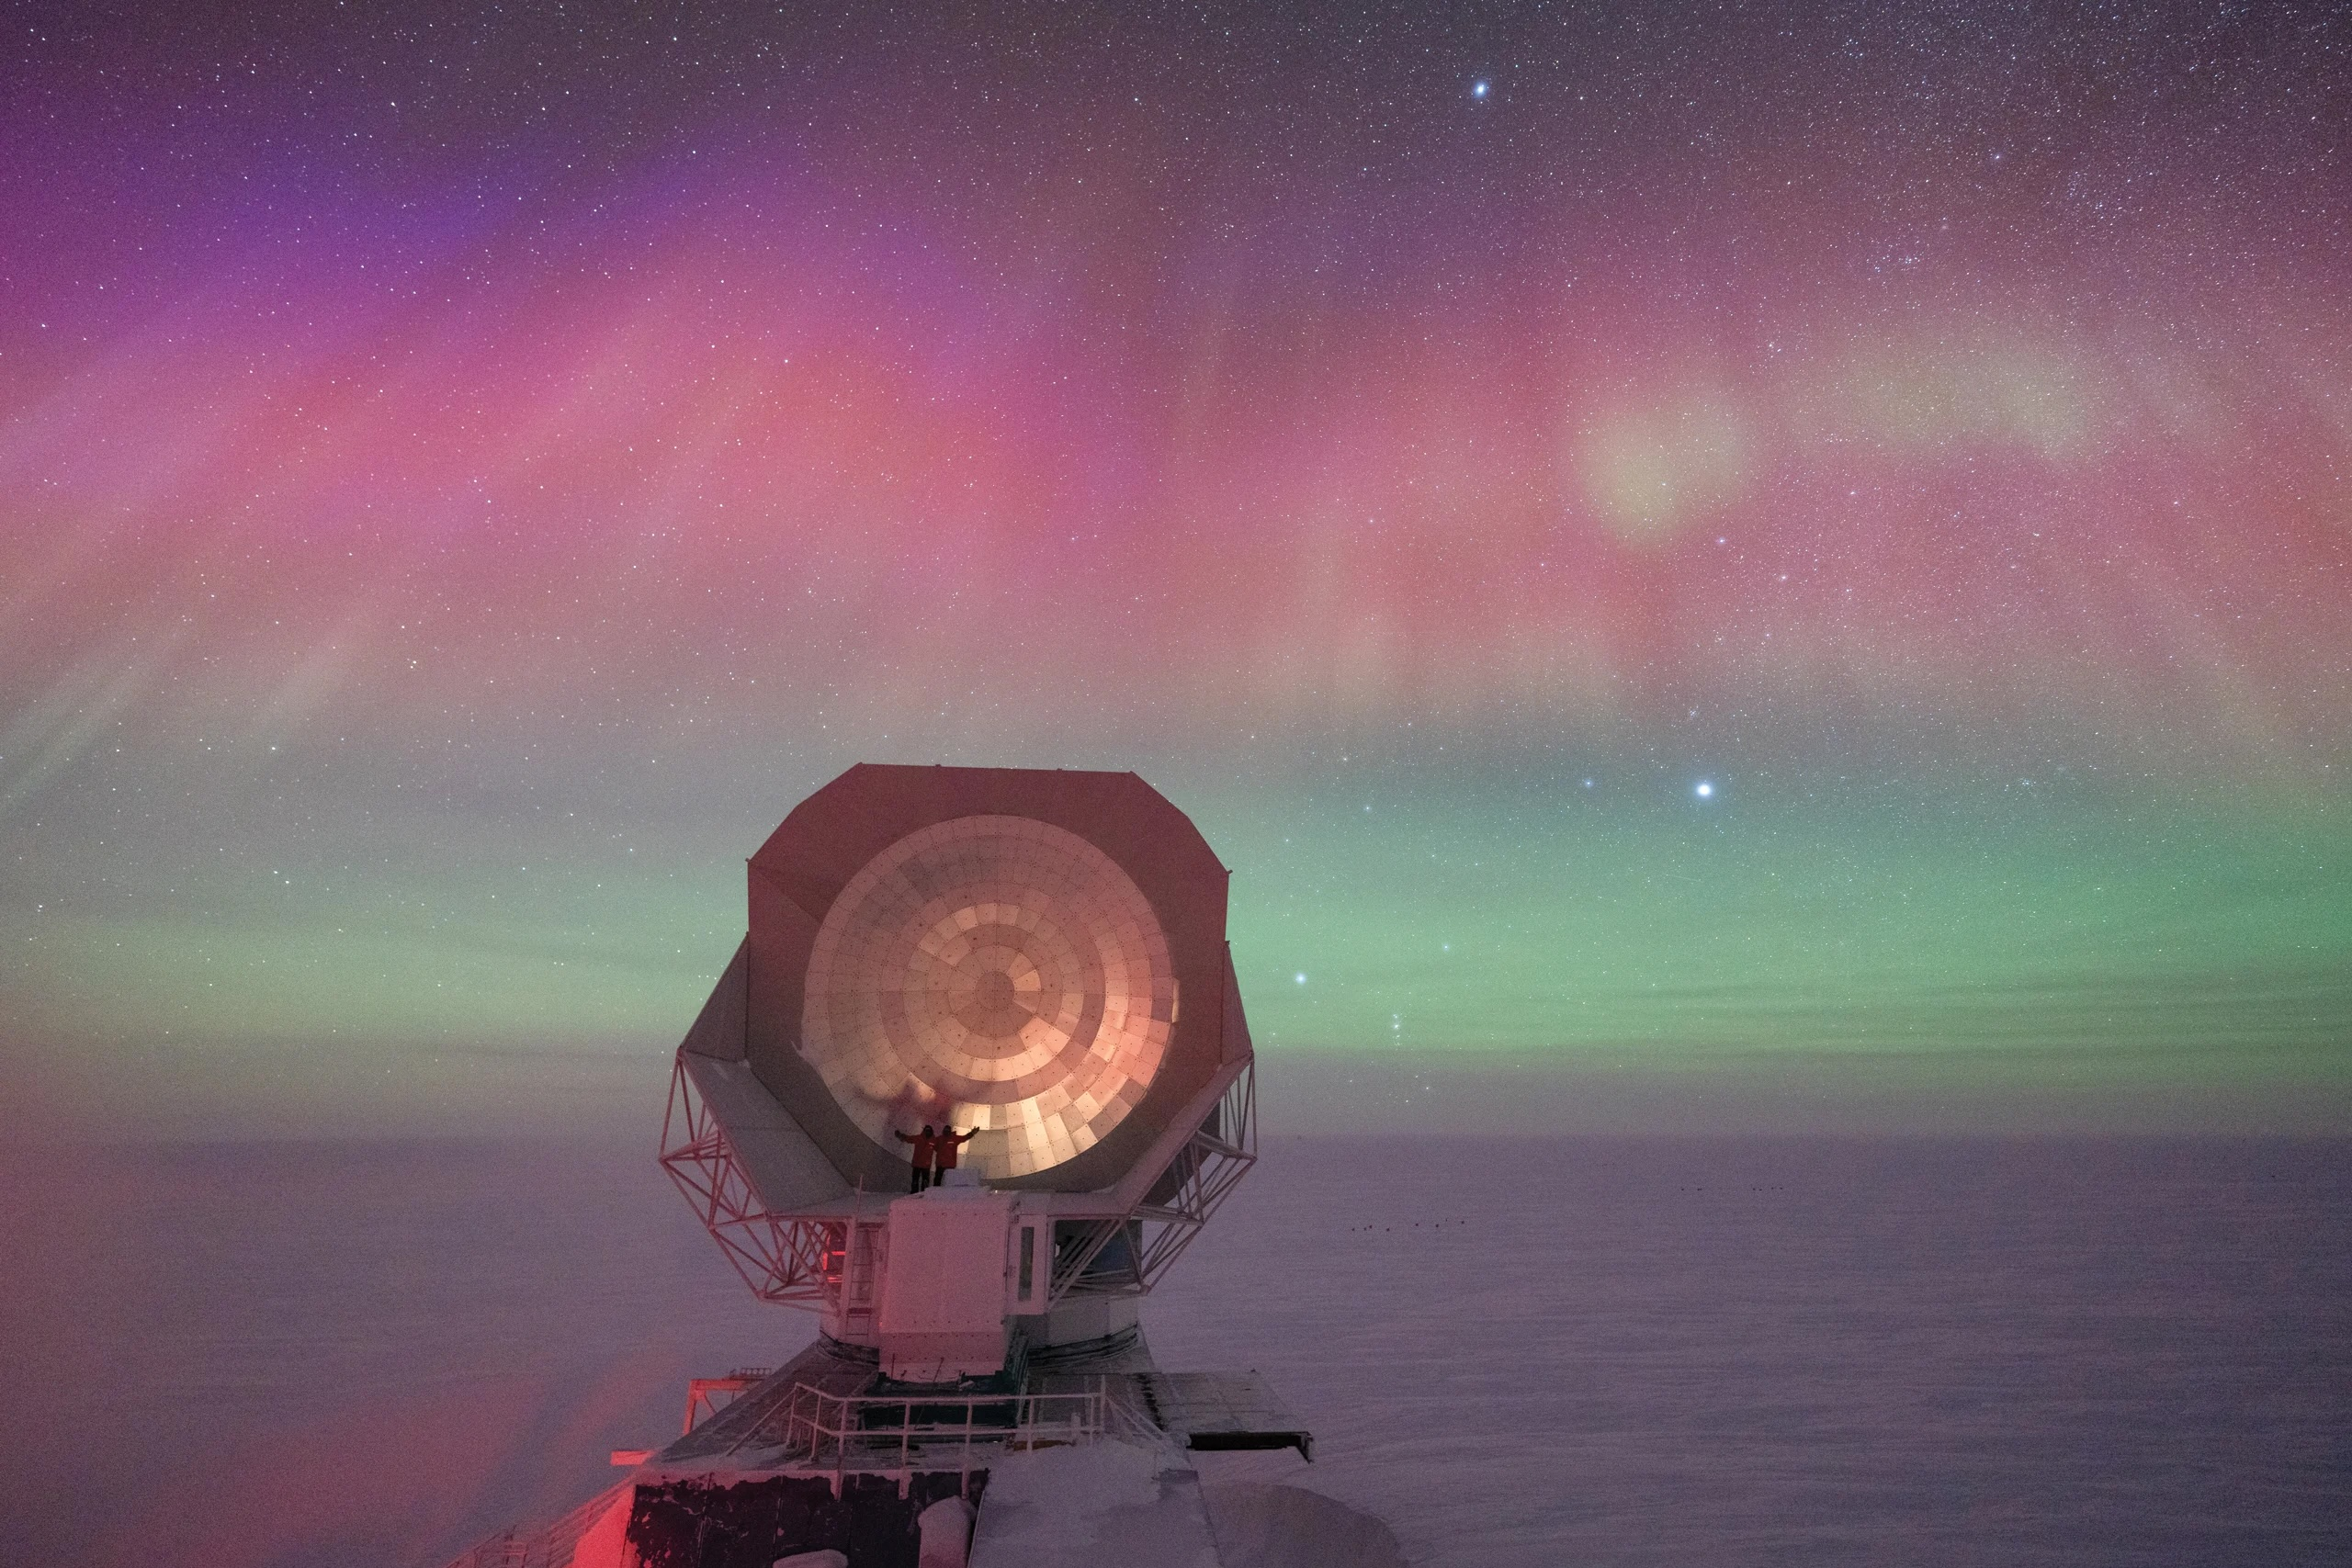
\includegraphics[width=0.8\textwidth]{imagen.jpeg}
\end{figure}

\subsection{Tablas}
Finalmente, en esta sección analizamos el trabajo con tablas.

\begin{table}[H]
  \centering
  \caption{Esta es una tabla sencilla y centrada.}
  \label{tab:EjemploSencillo}
  \begin{tabular}{c|ccc|c}
    & D1 & D2 & D3 & Oferta $\downarrow$ \\
    \hline
    F1 & 123 & 254 & 316 & 3600 \\
    F2 & 214 & 164 & 323 & 4500 \\
    F3 & 364 & 251 & 174 & 2800 \\
    \hline
  \end{tabular}
\end{table}

\begin{table}[H]
\centering
\caption{Tabla con celdas coloreadas}
\label{tab:colorCell}
\begin{tabular}{c|ccccc|c}
& D1 & D2 & D3 & D4 & DF & Oferta \\
\hline
S1 & 23 & 29 & 23 & 24 & \cellcolor{orange} 90 & 300 \\
S2 & 25 & 27 & 27 & 28 & \cellcolor{orange} 90 & 200 \\
S3 & 28 & 34 & 35 & 33 & \cellcolor{orange} 90 & 200 \\
S4 & 31 & 33 & 37 & 27 & \cellcolor{orange} 90 & 300 \\
\hline
Dem & 200 & 150 & 300 & 250 & \cellcolor{orange} 100 & \mbox{1000/1000} 
\end{tabular}
\end{table}

Me parece que babel en español le pone "Cuadro" a las tablas. Whatever. 

Para tablas más complicadas (y que usan multirow y cellcolor) puedes ayudarte de la página \href{https://www.tablesgenerator.com}{tables generator}.

\end{document}
